
\documentclass[./main.tex]{subfiles}


\begin{document}


\section{Travel}

\begin{frame}
\vfill
\centering
\begin{beamercolorbox}[sep=8pt,center,shadow=true,rounded=true]{title}
    \usebeamerfont{title} Analizu serwisu Travel
\end{beamercolorbox}
\vfill
\end{frame}

\begin{frame}{Charakterystyka serwisu}

Tematyką serwisu \url{www.travel.stackexchange.com} jest podróżowanie. Użytkownicy wymieniają się na nim informacjami na temat ciekawych miejsc, sposobów transportu i noclegów.
    
\end{frame}

\begin{frame}{Pytania badawcze}
    W ramach pracy badawczej postawiono następujące pytania:
    \begin{enumerate}
        \item jaki był wpływ pandemii COVID-19 na podróżowanie?
        \item które państwa najmocniej odczuły skutki pandemii?
        \item jak zmienił się poziom zaangażowania użytkowników forum? 
    \end{enumerate}
\end{frame}

\begin{frame}{Wpływ pandemii na podróżowanie}
\begin{center}
    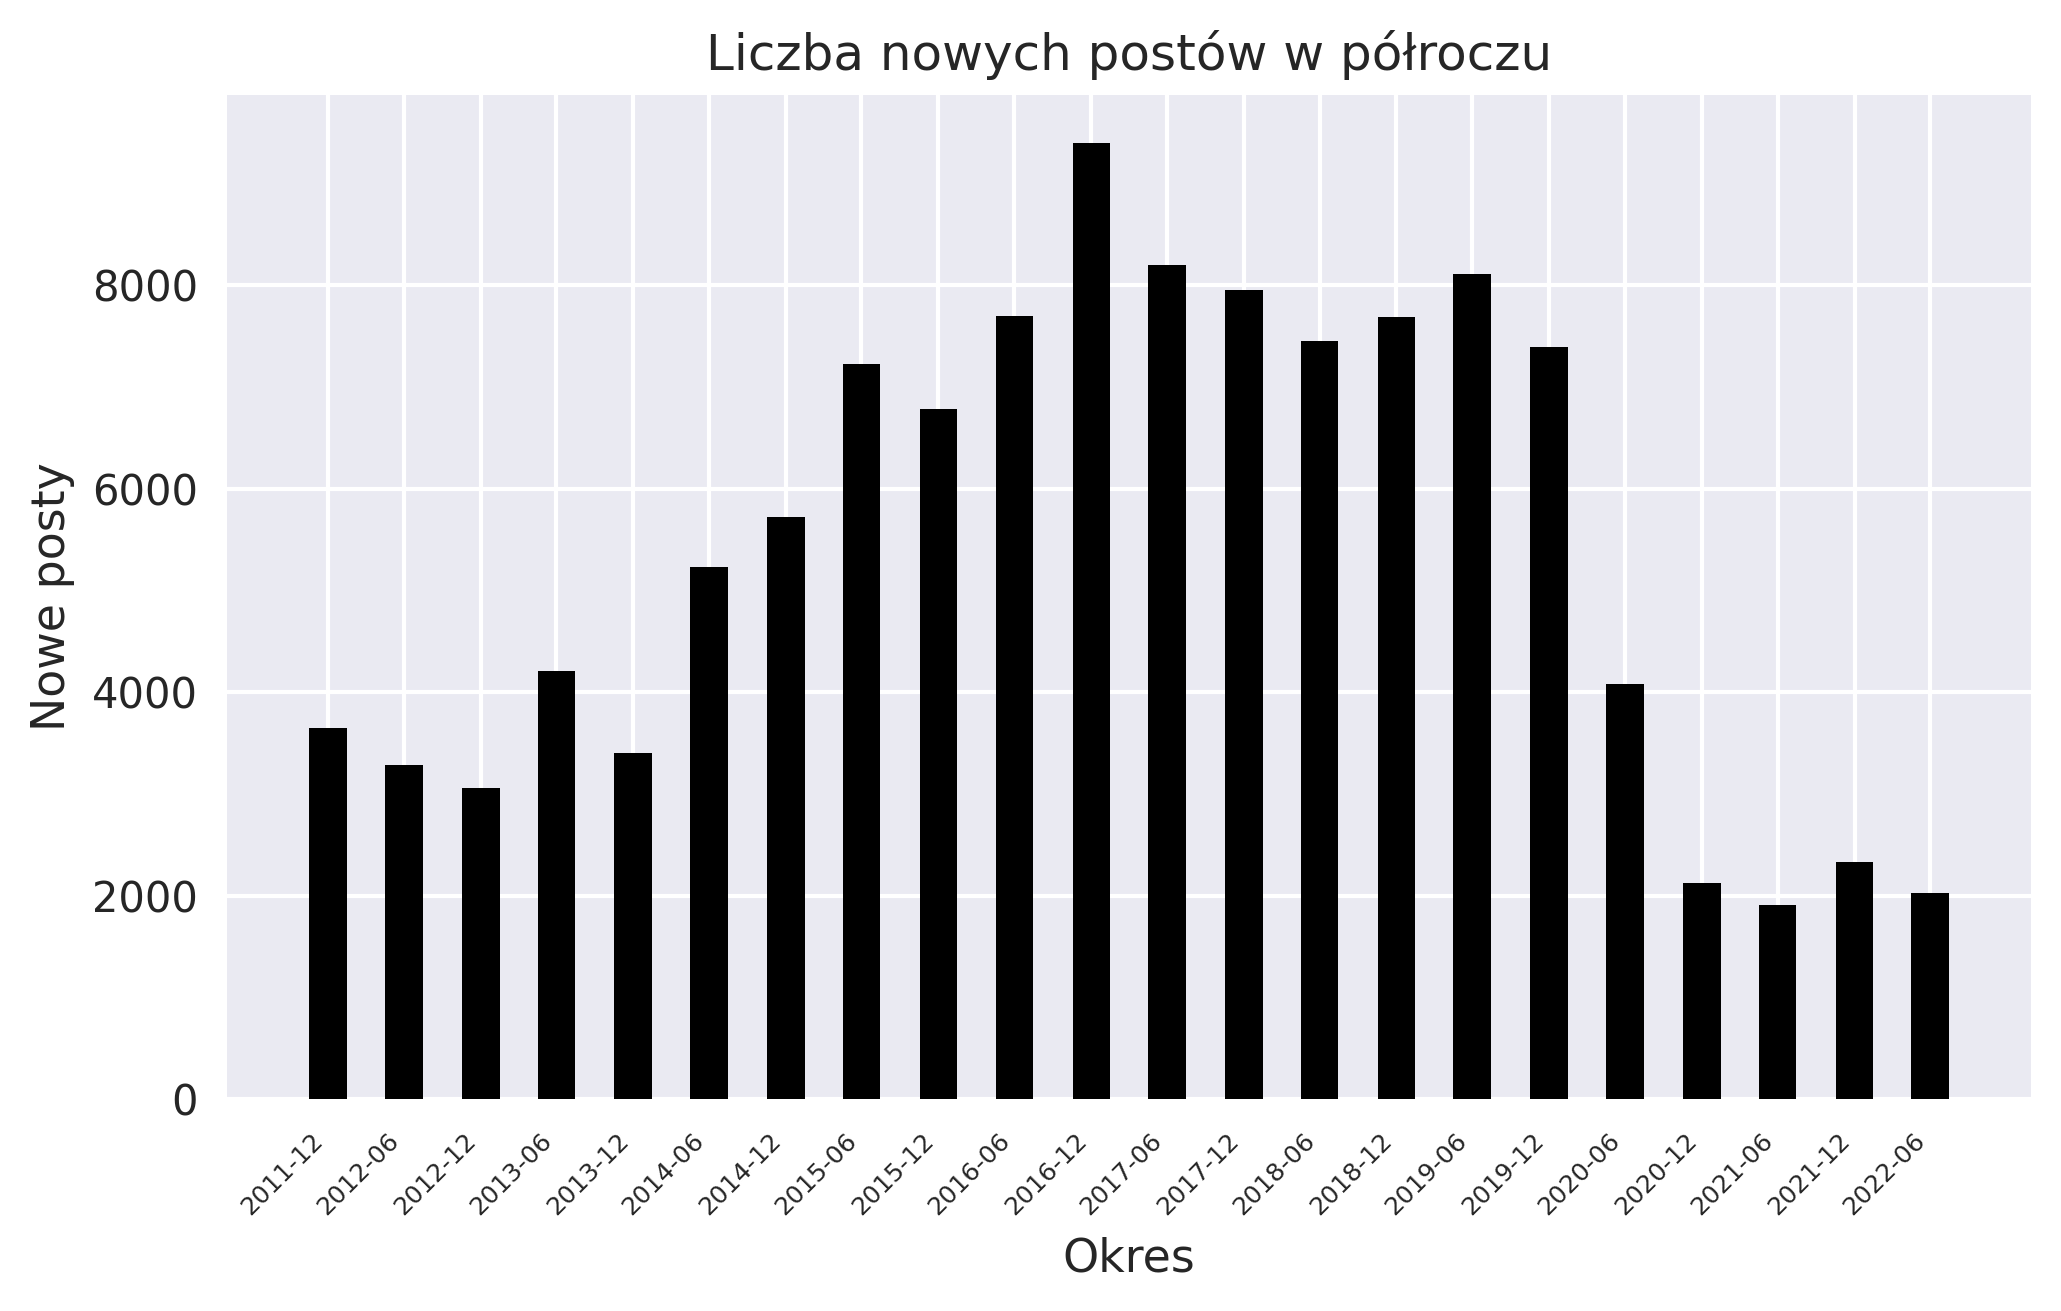
\includegraphics[width=\textwidth]{travel/new-posts.png}
\end{center}
\end{frame}

\begin{frame}{Wpływ pandemii na podróżowanie (c.d.)}
\begin{center}
    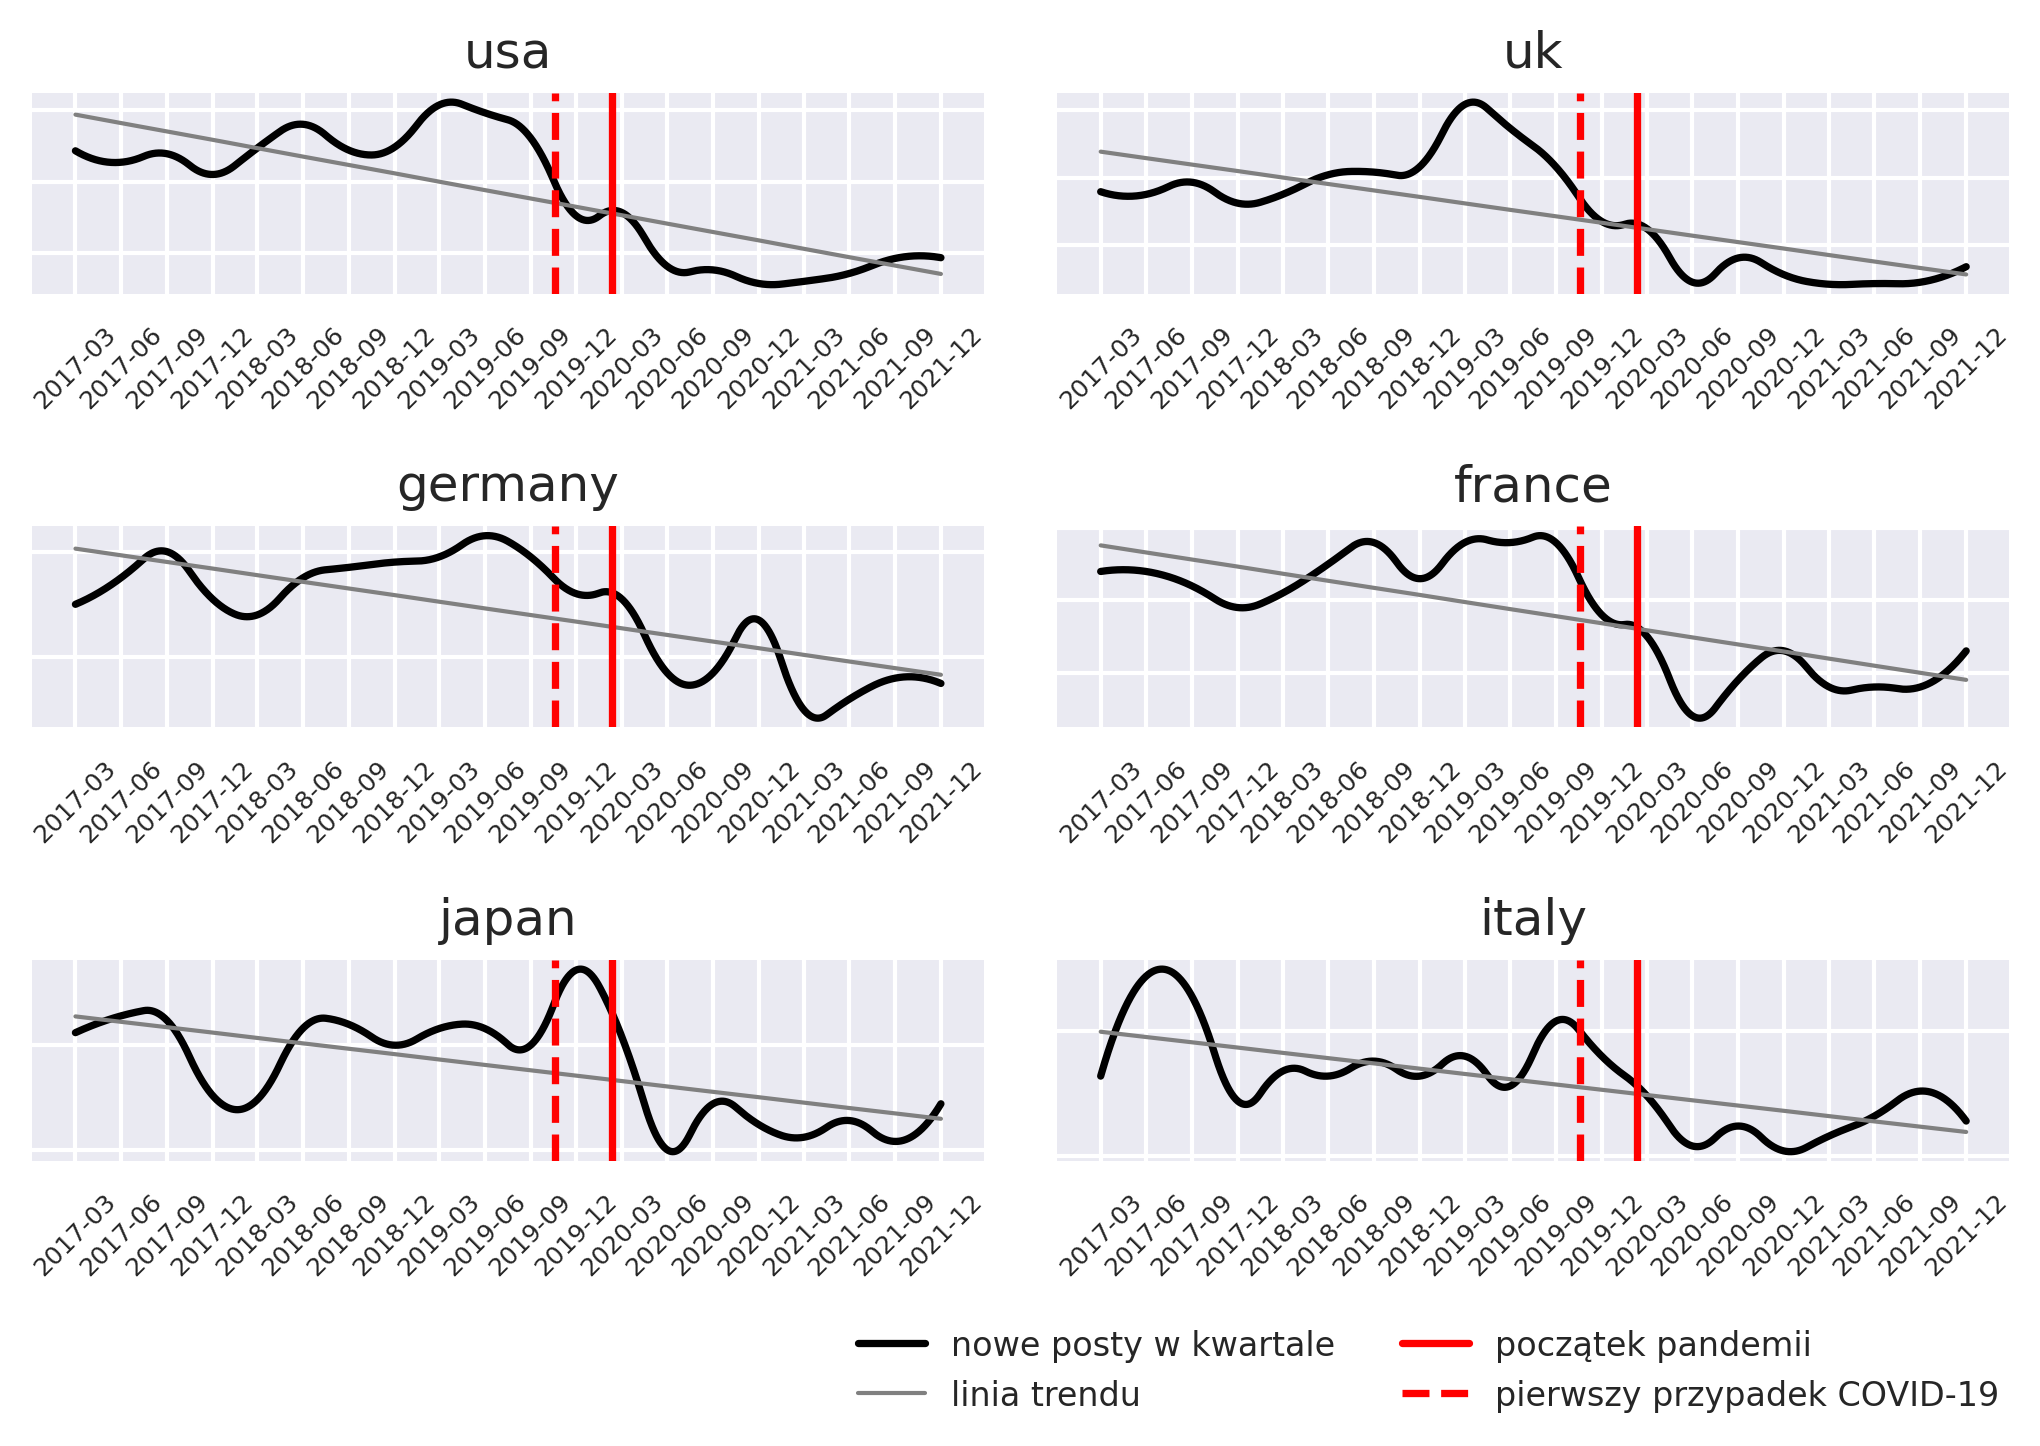
\includegraphics[width=\textwidth]{travel/countries.png}
\end{center}
\end{frame}

\begin{frame}{Wpływ pandemii na podróżowanie (c.d.)}

Poniżej przedstawiono współczynniki kierunkowe linii trendu dla 6 najpopularniejszych krajów: 

\begin{center}
    \begin{table}[htb]
    \begin{tabularx}{\linewidth}{CC}
    \begin{tabular}{|l|l|}
    \hline
    \textbf{Kraj}    & \textbf{wsp. kier.}     \\ \hline
    usa     & -11.68 \\ \hline
    uk      & -9.56  \\ \hline
    japan   & -1.28  \\ \hline
    germany & -1.25  \\ \hline
    italy   & -1.05  \\ \hline
    france  & -0.98  \\ \hline
    \end{tabular} 
    \caption*{Metoda regresji liniowej}
    &
    \begin{tabular}{|l|l|}
    \hline
    \textbf{Kraj}    & \textbf{wsp. kier.} \\ \hline
    usa     & -11.1 \\ \hline
    uk      & -8.69 \\ \hline
    japan   & -1.18 \\ \hline
    germany & -1.16 \\ \hline
    italy   & -0.96 \\ \hline
    france  & -0.89 \\ \hline
    \end{tabular}
    \caption*{Mann-Kendall Trend Test}
    \end{tabularx}
    \end{table}
\end{center}
\end{frame}


\begin{frame}{Wpływ pandemii na podróżowanie - wnioski}
    \begin{enumerate}
        \item z powodu pandemii największy spadek popularności na forum zanotowały USA i UK (może to wynikać z tego, że forum jest angielskojęzyczne)
        \item u pozostałych państw stwierdzono podobne do siebie spadki
        \item dla większości państw, w okresie między pierwszym zachorowaniem na COVID a ogłoszeniem pandemii liczba nowych postów była stała
    \end{enumerate}
\end{frame}

\begin{frame}{Nowi użytkownicy forum}
    \begin{center}
    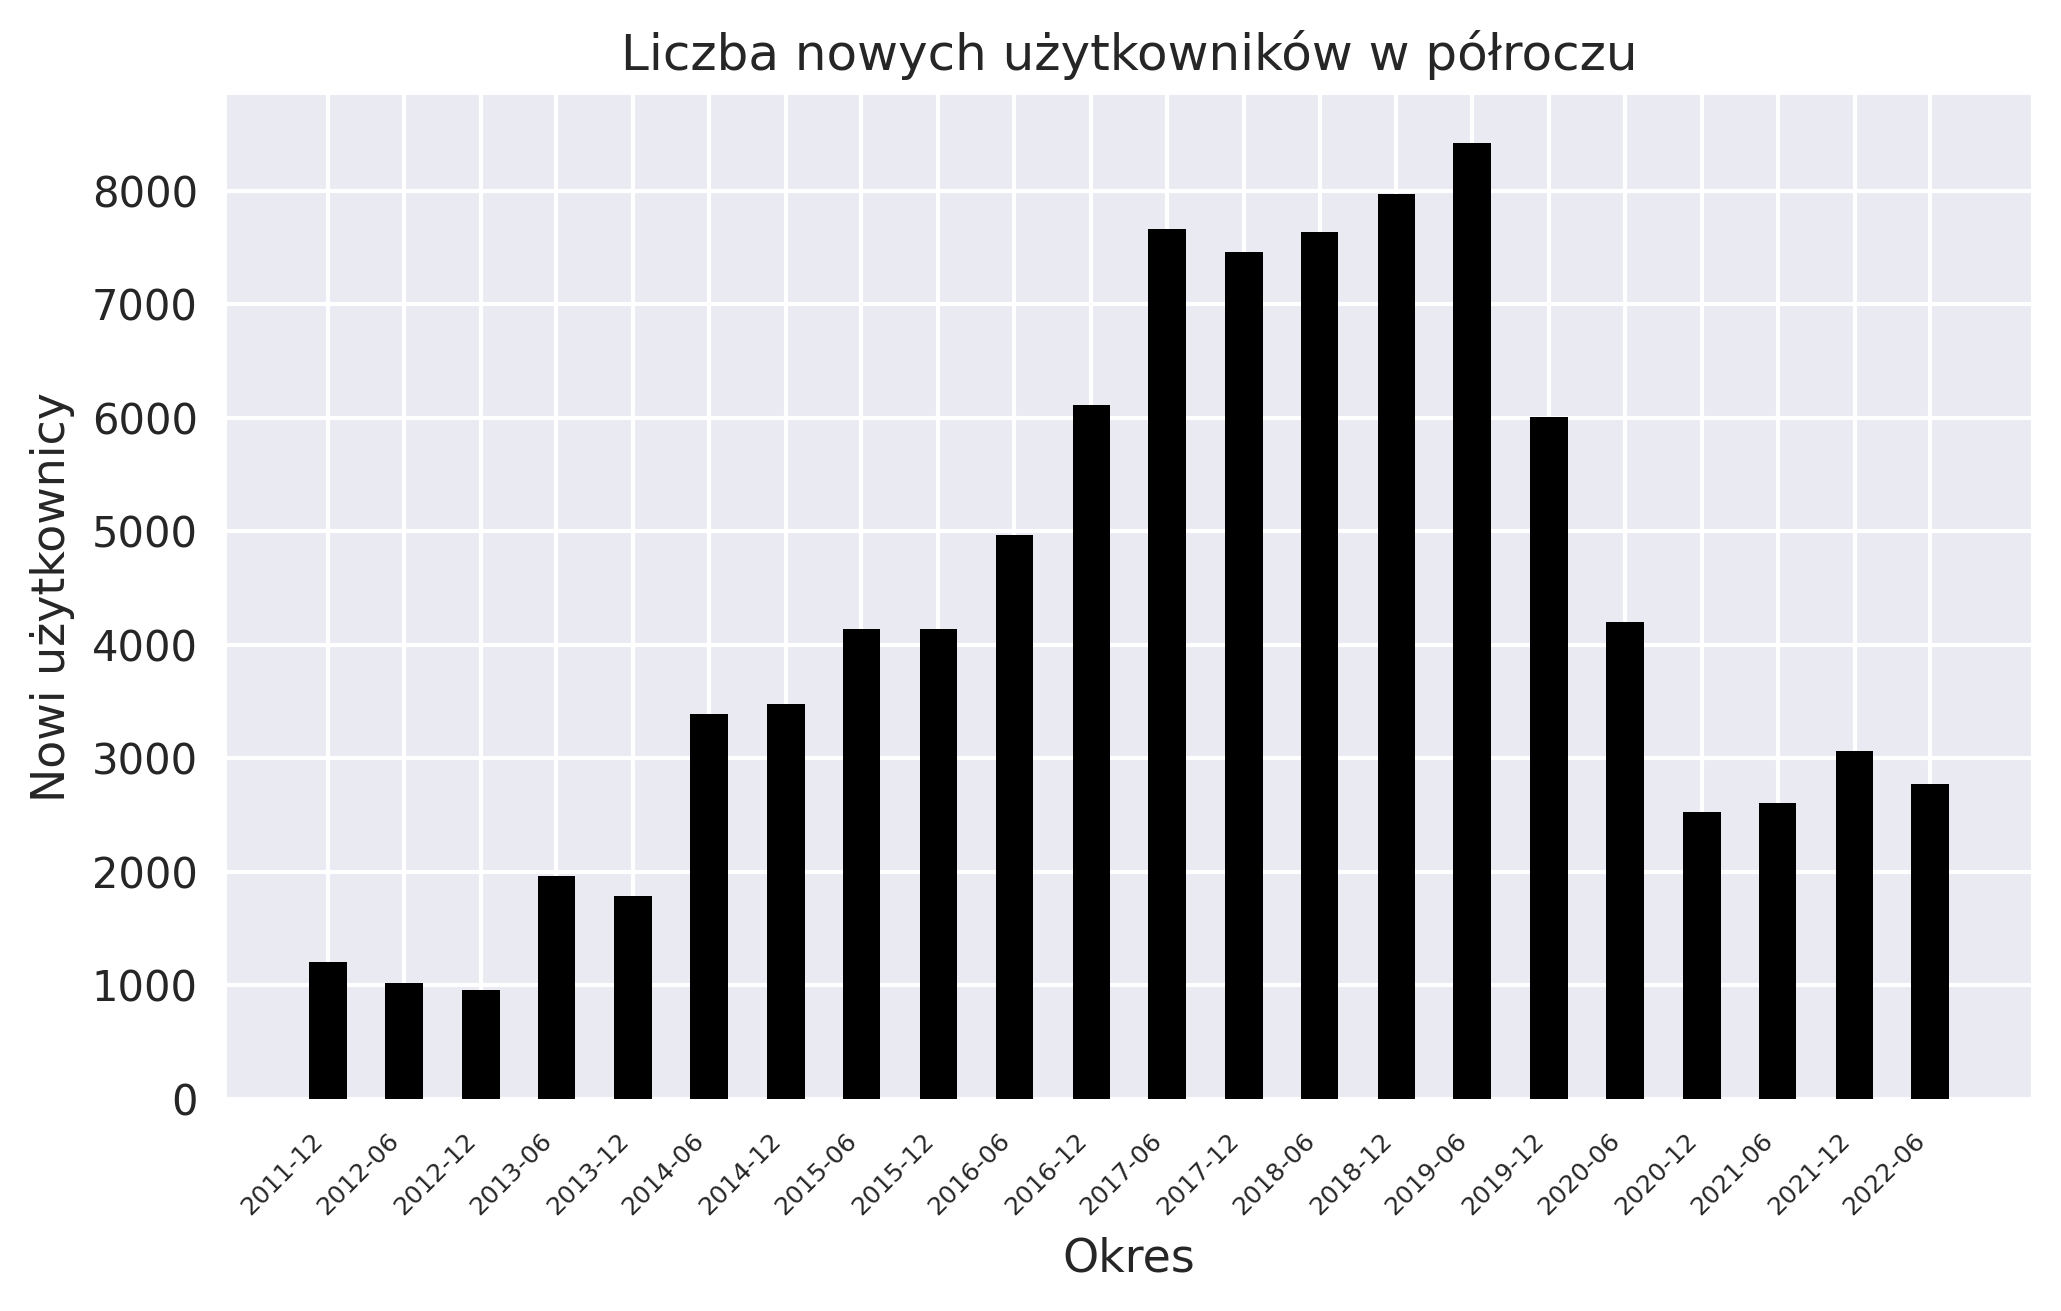
\includegraphics[width=\textwidth]{travel/new-users.png}
    \end{center}
\end{frame}

\begin{frame}{Zaangażowanie użytkowników}
    \begin{center}
    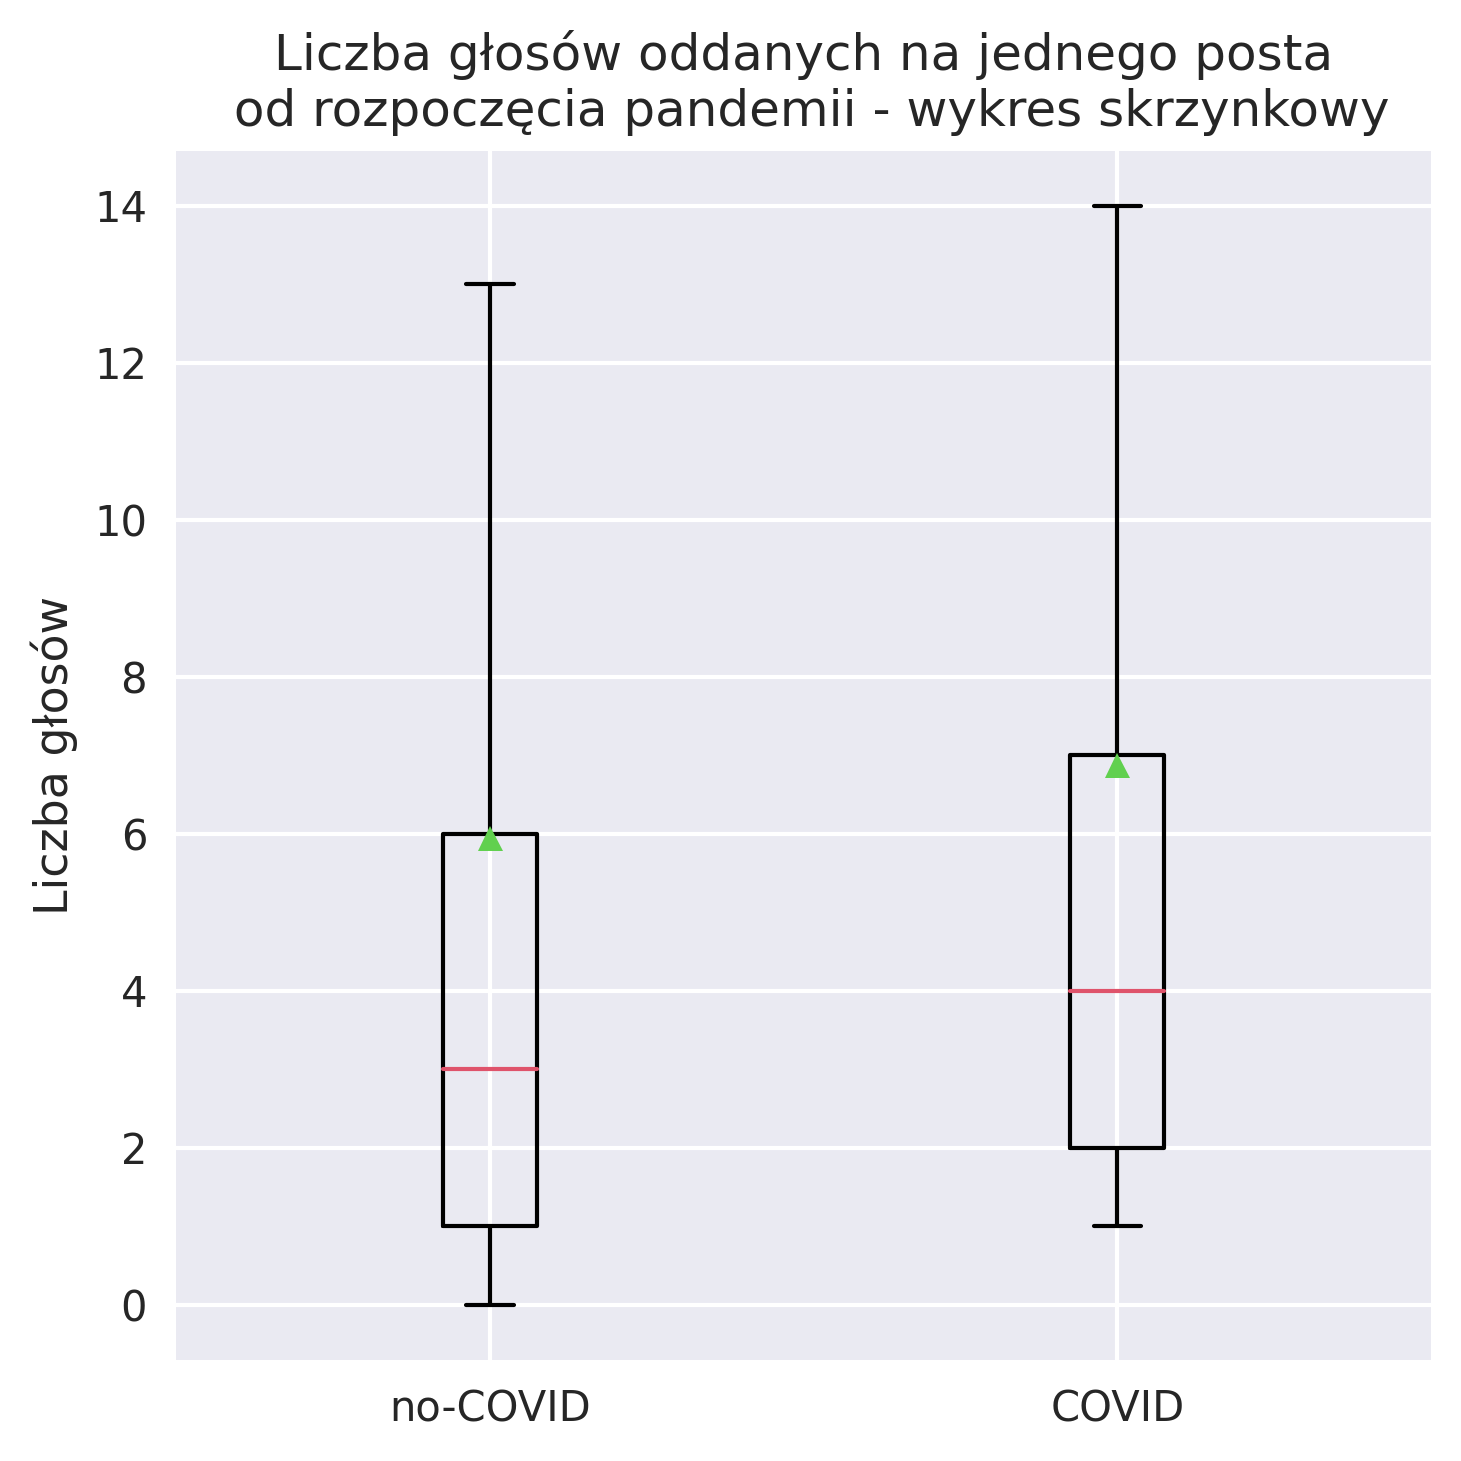
\includegraphics[height=0.67\textheight]{travel/votes.png}
    \end{center}
    Posty zawierające wzmiankę o COVID cieszą się większym zainteresowaniem niż posty bez odniesień do pandemii. 
\end{frame}

\end{document}